\chapter{Languages and Computability}\label{berekenbaarheid}


\section{The Turing Machine as a Decider or Recognizer}\label{turingmachines}

In the previous sections, we looked at two classes from the Chomsky
hierarchy. In particular we studied the machines that decide the
membership problem for these languages: whether a given string belong to
a given language. We already understand that some (many?) languages
are beyond the decision power of DFAs, PDAs, and even LBAs. So it is
time to start studying machines that can do more. We use Turing
machines.

Roughly speaking, a TM has a two infinite (unlimited would be enough)
\marton{maybe a short explanation of what two infinite and unlimited are would be nice here}
tape consisting of squares (or cells) with one symbol each, a control
unit, a tape head that can read the symbol in a square, and write a
new one. The action of the machine depends on the internal state of
its control unit and the symbol being read. Possible actions are:
writing a symbol and moving the tape head. Figure~\ref{turing1} shows
the parts of the machine and the actions that are described by a
function $\delta$.


\begin{figure}[h]
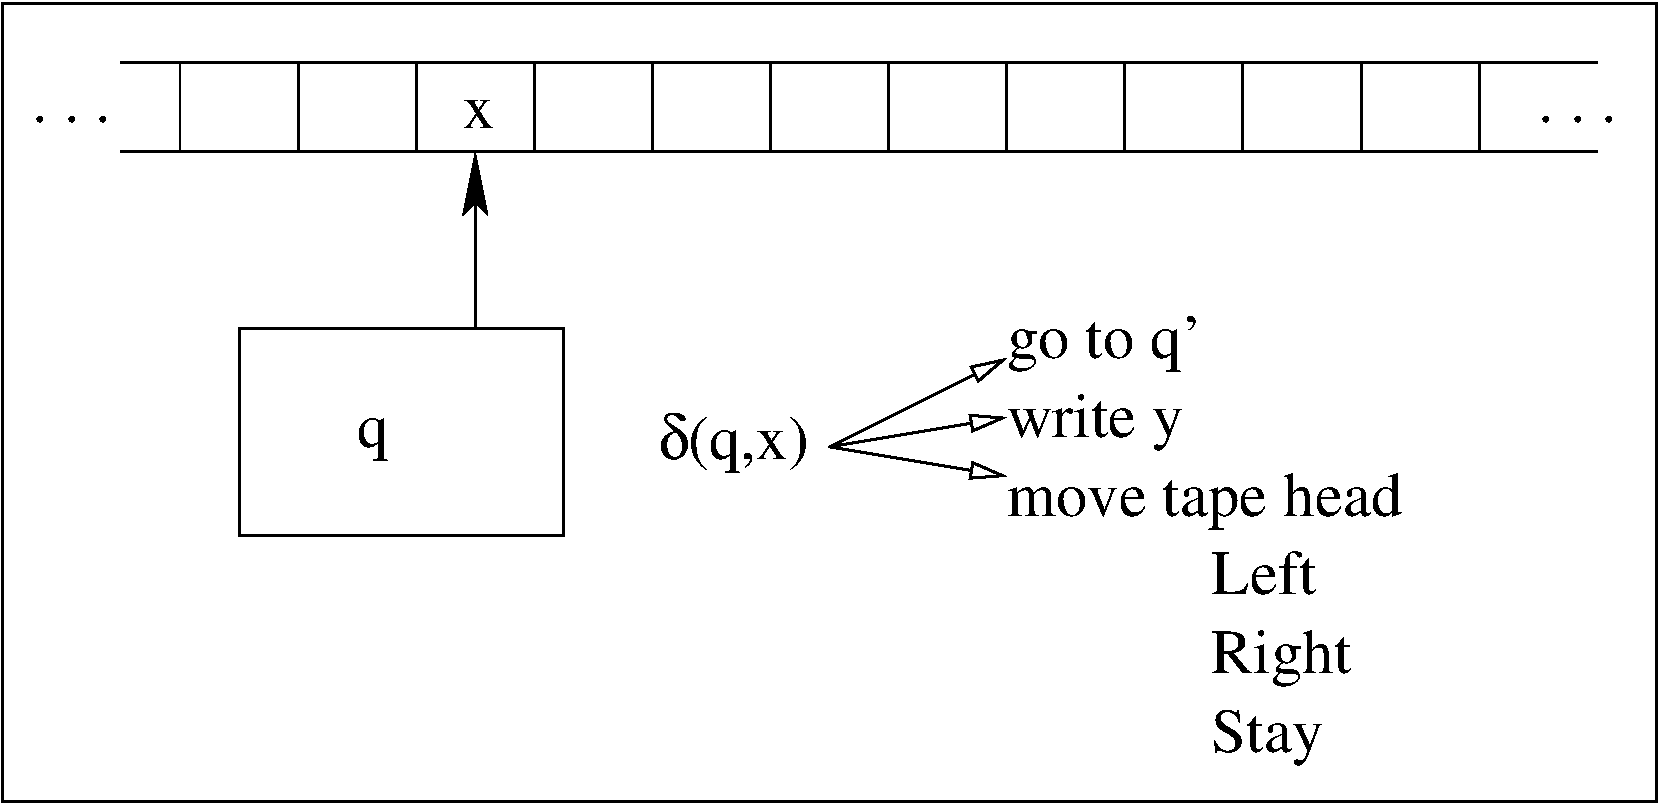
\includegraphics[%
  width=0.6\linewidth,
  keepaspectratio]{turing1eng}
\caption{Schema of a Turing machine\label{turing1}}
\end{figure}

\vspace{-5cm}\hspace{10cm}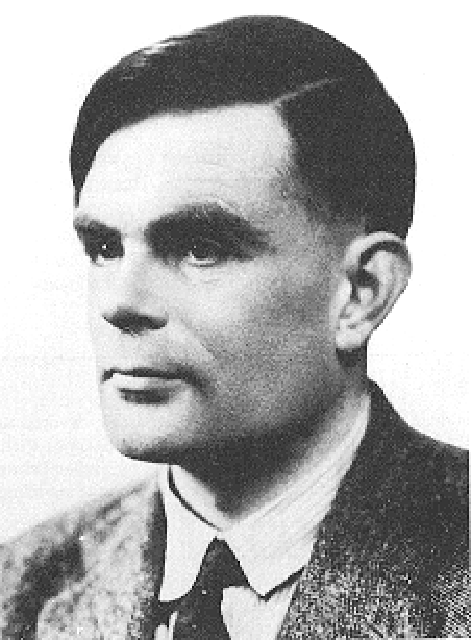
\includegraphics[%
  width=0.2\linewidth,
  keepaspectratio]{static/turing}

\vspace{0.5cm} More formally:

\begin{definition}[Turing Machine]
A {\bf Turing Machine} is a 7-tuple
%
$(Q, \Sigma, \Gamma, \delta, q_s, q_a, q_r)$
%
with $Q, \Sigma, \Gamma$ finite sets:

\begin{itemize}
\item
Q is the set of states

\item
$\Sigma$ is an input alphabet not containing \#

\item
$\Gamma$ is the tape alphabet; $\# \in \Gamma$ and $\Sigma \subset \Gamma$

\item
$q_s$ is the start state

\item
$q_a$ is the accepting end state


\item
$q_r$ is the rejecting end state and different from $q_a$


\item
$\delta$ is the transition function: it is a total function with
  signature

$~~~~~~~~~~Q \times \Gamma \rightarrow Q \times \Gamma \times \{L,R,S\}$

where $L, R, S$ denotes the direction the tape head moves after the transition (left, right, stay)

\end{itemize}
\end{definition}

The machine is initialized as follows:
\begin{itemize}
\item the symbols of a string from $\Sigma^*$ are put in subsequent
tape cells: they constitute the input string; all other cells contain
\#
\item the machine is put in start state $q_s$
\item the tape head is positioned at the leftmost symbol of the input
  string; if the input string is empty, it can be positioned anywhere
\end{itemize}

The machine works as follows: on the basis of the state of the
machine and the symbol under its head, $\delta$ determines the next
state of the machine, which symbol needs to be written, and the
direction of the head movement. This is repeated until
\begin{itemize}
\item the machine arrives in the state $q_a$: the input string is
  accepted and sometimes, the contents of the tape at this moment are
  considered the result of the computation
\item the machine arrives in the state $q_r$: the input string is
 rejected
\item neither of the above, and it continues ... the machine {\em
  loops} or is in an infinite loop
\end{itemize}

As with DFA and PDAs, there are alternative definitions of TMs, or
variants. Here are a few that do not seem to matter: they define {\em
  equivalent} machines. You can prove that, but you must start by
defining precisely what you mean by equivalent.

\begin{itemize}
\item the tape head can not stay at the same place: it must at every step move left of right
\item there can be more than one accepting or rejecting state
\item the tape is unlimited in only one direction (it is half-infinite)
\item there is more than one tape
\item the input alphabet has only two symbols\label{twosymbols}
\item there are only three states
\item the machine has two stacks instead of a tape
\end{itemize}

About the symbol \#: initially it indicates that a tape cell has not
been visited or written before, but the machine may write that symbol
any time. Often, texts refer to it as the blank symbol and use
$\sqcup$. We often refer to \# as the blank symbol as well.


For a given TM, $\Sigma^*$ consists of three disjunct subsets:
\begin{enumerate}
\item the strings accepted by TM: $L_{TM}$
\item the strings for which TM loops: $\infty_{TM}$
\item all other strings (they are rejected)
\end{enumerate}
These subsets are used in the following definitions.

% \clearpage

\begin{definition}[To recognize]
A Turing machine TM recognizes $L_{TM}$.
\end{definition}

Its complementary definition is

\begin{definition}[Turing recognizable language]
A language L is Turing recognizable if there exists a Turing Machine
TM so that TM recognizes $L$ or alternatively, $L = L_{TM}$
\end{definition}

Here is an example of a recognizable language L and a TM that
recognizes L: $\Sigma = \{a,b\}$, $L = \{a\}^*$. Table \ref{turing3}
describes $\delta$.

\begin{table}[ht]
\center
\begin{tabular}{|l|c||l|c|c|}
\hline
$Q$    & $\Gamma$   &  $Q$  &  $\Gamma$ &  LRS \\ \hline
$q_s$  &  a         &  $q_s$&   \#      &  R   \\
$q_s$  &  b         &  x    &    b      &  S   \\
$q_s$  &  \#        &  $q_a$&    -      &  -   \\
x      &  a         &  x    &    a      &  S   \\
x      &  b         &  x    &    b      &  S   \\
x      &  \#        &  x    &    \#     &  S   \\
\hline
\end{tabular}
\caption{A TM recognizing $\{a\}^*$} \label{turing3}
\end{table}
$\infty_{TM}$ is not empty: every string not in L brings the machine
in an infinite loop. But we can also construct a TM for L that always
halts, this is shown in table \ref{turing4}.

\begin{table}[ht]
\center
\begin{tabular}{|l|c||l|c|c|}
\hline
$Q$    & $\Gamma$   &  $Q$  &  $\Gamma$ &  LRS \\ \hline
$q_s$  &  a         &  $q_s$&   \#      &  R   \\
$q_s$  &  b         &  $q_r$&    -      &  -   \\
$q_s$  &  \#        &  $q_a$&    -      &  -   \\
\hline
\end{tabular}
\caption{A TM that decides $\{a\}^*$} \label{turing4}
\end{table}

This distinction is captured in the following definitions:

\begin{definition}[To decide]
A Turing Machine TM decides a language L, if TM recognizes L and
$\infty_{TM} = \emptyset$
\end{definition}

\begin{definition}[Turing decidable language]
A language L is Turing decidable if there exists a Turing Machine that
decides L.
\end{definition}

It might not be clear at this point that to recognize and to decide
are two very different things, but we will work towards this
understanding. Still, it should be clear that a decidable language is
also recognizable.

Other terminology for {\em decidable language} is {\em recursive
  language}, and for {\em recognizable language}, one uses {\em
  recursively enumerable}, or sometimes {\em semidecidable}.

\begin{definition}[Co-recognizable/co-decidable]
A language L is \textbf{co-recognizable/co-decidable} if $\overline{L}$
is recognizable/decidable.
\end{definition}

\begin{theorem} \label{corecognizable}
If L is decidable, then L is also co-decidable.
\end{theorem}
\begin{proof}
Let M be the TM deciding L; now switch the roles of $q_a$ and $q_r$.
\end{proof}

\begin{theorem} \label{isdec}
If L is recognizable and co-recognizable, then L is decidable.
\end{theorem}
\begin{proof}
Let M1 be the machine that recognizes L, and M2 the machine
recognizing $\overline{L}$. The idea is to have a machine M that
lets M1 and M2 run in parallel: as soon as M1 accepts, accept; as soon
as M2 accepts, reject. M1 and M2 can not accept both, and for any
given string, at least one of them halts in the accepting state. This
M decides L.

The definition of M is informal, and we should make it more formal:
define M as a 2-tape machine and work out the details.
\end{proof}

\begin{theorem}
Some languages are not recognizable.
\end{theorem}
\begin{proof}
The set of Turing Machines is countably infinite, so the set of
recognizable languages can be at most countably infinite. On the other
hand, the set of languages (being ${\cal P}(\Sigma^*)$) is uncountably
infinite. So there must exist languages that are not recognizable.
In fact, most languages are not recognizable.
\end{proof}

What is our plan with Turing Machines?

\begin{itemize}
\item we want to further explore the difference between deciding and
  recognizing
\item fit into this picture the regular and context free
  languages
\item study examples of languages that can not be decided or
  recognized by a TM and general techniques for proving this
\end{itemize}



\paragraph{Selfie:} Comment on the following sentences:

\begin{itemize}
\item every string is recognizable
\item every string is decidable
\item every finite language is decidable/recognizable
\item the union/intersection of two recognizable languages is recognizable
\item the intersection of a recognizable and a decidable language is
  decidable
\end{itemize}




% \clearpage
\section{A graphical representation of Turing Machines}

Just as FSAs and PDAs, TMs can be visualized by a graph: the vertices
are the states. Figure~\ref{turing2} illustrates it for the TM
deciding the language $\{0^n1^n|n \geq 0\}$.




\begin{figure}[h]
\begin{center}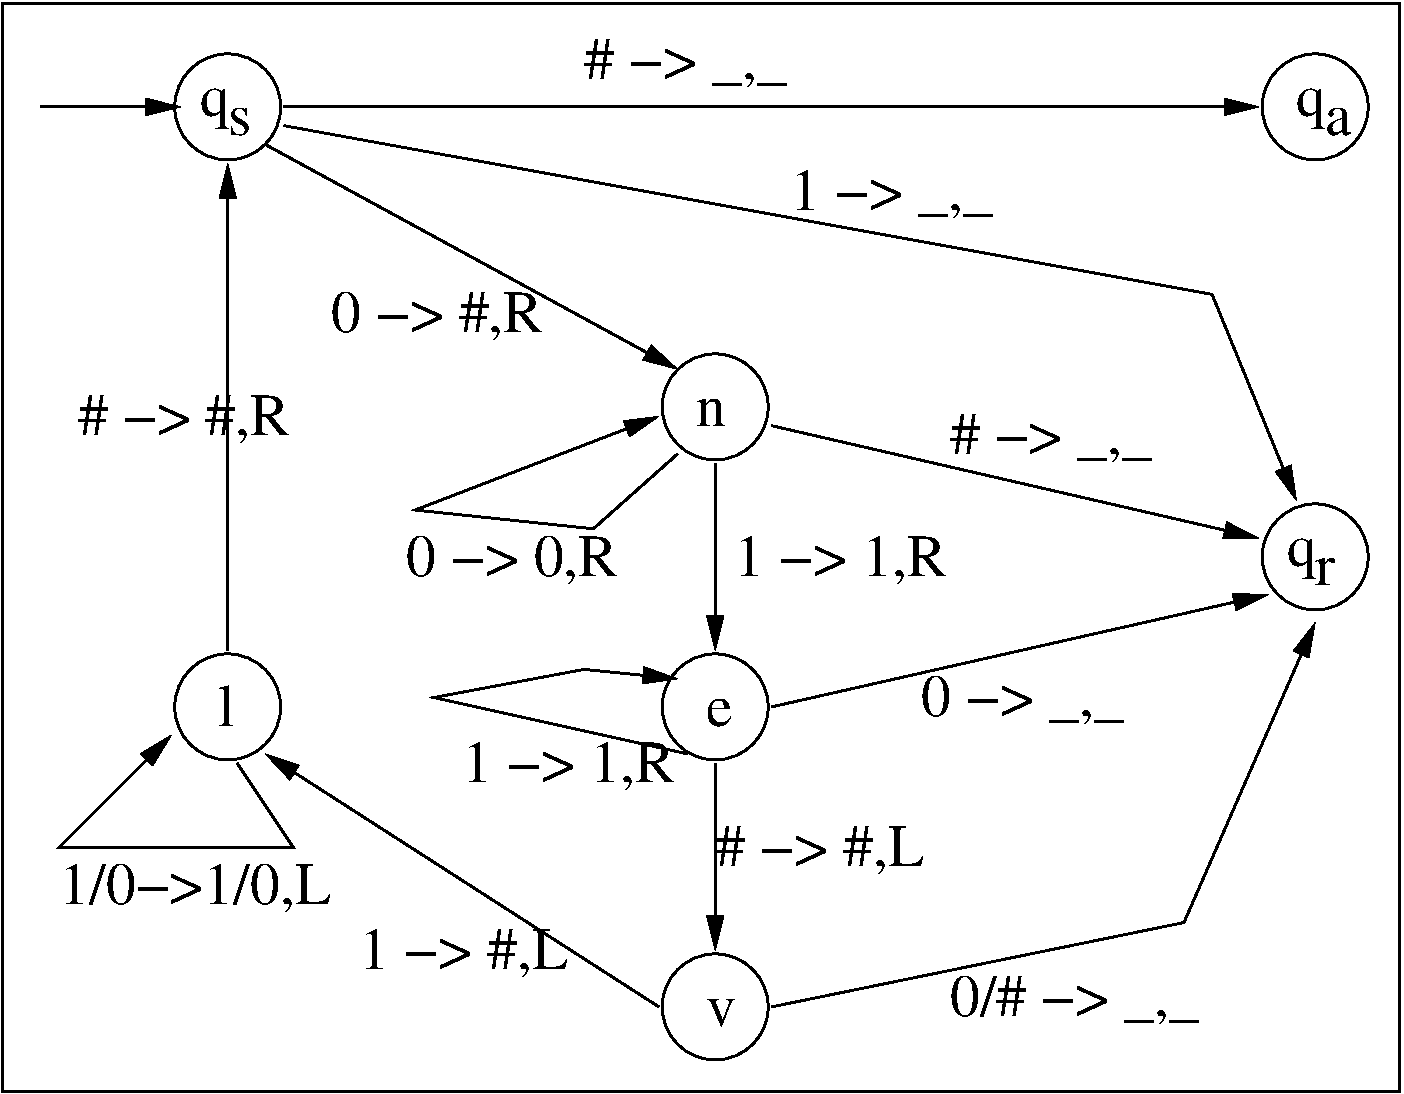
\includegraphics[%
  width=0.7\linewidth,
  keepaspectratio]{turing2}\end{center}
\caption{Graphical representation of a Turing Machine\label{turing2}}
\end{figure}

Each state has as many outgoing edges as elements in $\Gamma$ (some
parallel edges are treated together) - except for the accepting and rejecting
state of course. The label represents the $\delta$ of the machine. We
use \_ to indicate that the value at this place is irrelevant: this is
typical for transitions to a halting state.

% \clearpage

One can describe in words what the machine does with an input
consisting of only zeroes and ones.

\begin{itemize}
\item if in the start state the head sees a
\begin{itemize}
\item \#: accept
\item 1: reject
\item 0: wipe it out, go to the right, and switch to state $n$; it
  will skip all zeroes
\end{itemize}

\item if in state $n$ the head sees a
\begin{itemize}
\item \#: reject
\item 1: go right to state $e$; it will skip all ones
\item 0: go right
\end{itemize}


\item in state $e$
\begin{itemize}
\item 1: go right
\item 0: reject
\item \#: go left, switch to $v$; it will erase one 1
\end{itemize}

\item in state $v$
\begin{itemize}
\item 0: reject (but actually can't occur)
\item \#: reject (but actually can't occur)
\item 1: erase the 1 (overwrite it by \#); go left on the tape and to
  state $l$; it will find the leftmost symbol of the string
\end{itemize}

\item in $l$
\begin{itemize}
\item 0/1: go left;
\item \#: go right and to the start state
\end{itemize}

\end{itemize}

As you see, every state has its little something to contribute to the
whole program.


The TM in Figure~\ref{turing2} proves that
%
$\{0^n1^n|n \geq 0\}$ is a decidable language.

\marton{Does this TM really decide $0^n1^n$ and not $0+1+|\epsilon$?}

% \clearpage
\section{Representation and simulation of TM computations}

It is often handy to be able to compactly represent a {\em
  configuration} of a TM: it is like a computer memory dump, together
with all registers and the hardware state, so that execution could
restart from that information. For a TM, we can do that because at
each moment, only a finite part of the tape is in use, i.e. is
different from \#. So, a string of the form

$~~~~~~~~~~~~~~~~\alpha q \beta$

can represent the tape containing $\alpha\beta$ with to its left and
right only \#; moreover, the machine is in state $q$ and the head is
positioned under the leftmost symbol of $\beta$. $\alpha$ and $\beta$
may contain \#.

A start configuration is always of the form $q_s\alpha$, and an end
configuration is either $\alpha q_a \beta$ or $\alpha q_r \beta$.

During the execution of the TM, two successive configurations are
related by $\delta$ as follows:


$~~~~~~~~~~\alpha q b \beta$ \rpijl $\alpha p c \beta$ if $\delta(q,b) = (p,c,S)$

$~~~~~~~~~~\alpha a q b \beta$ \rpijl $\alpha p a c \beta$ if $\delta(q,b) = (p,c,L)$

$~~~~~~~~~~\alpha q b \beta$ \rpijl $\alpha c p \beta$ if $\delta(q,b) = (p,c,R)$

You can add some transitions for the case where $\alpha$ or $\beta$ is
empty: you might need to generate extra occurrences of \#.


A sequence of configurations from a start to an end configuration -
following $\delta$ - is called a {\em computation history}.

It is reasonably easy to see that the computation of any TM can be
simulated by a program, for instance in Prolog. To make that more
concrete, here is some Prolog code. A configuration $\alpha q \beta$
is represented as a term with principal functor conf/3, as follows:

$~~~~~~~~~~~~conf([a_n, ... , a_2,a_1],q,[b_1,b_2,...,b_m])$, where
$a_1a_2...a_n = \alpha$ and $b_1b_2...b_m = \beta$
%
\\ and $a_i, b_j \in \Gamma$.\footnote{Look up {\em Huet's Zipper}}

Here is part of the Prolog program working with configurations:

\begin{verbatim}
       onestep(conf(Alpha,Q,[]), NewConf) :-
                 onestep(conf(Alpha,Q,[#]), NewConf).
       onestep(conf(Alpha,Q,[B|Beta]), conf(Alpha,P,[C|Beta])) :-
                 delta(Q,B,P,C,stop).
\end{verbatim}

\paragraph{Selfie:} Extend the above program, and explain in words the function of each clause.


We should also understand that a TM can simulate a Prolog program: to
do that directly would be a lot of work, so here is a classical road
towards the same goal. First prove that Prolog can be implemented on
an Intel machine - that has been done many times, e.g. by the SWI
Prolog implementation. Next prove that an Intel machine can be
simulated by a register machine; the register machine is in the first
place a theoretical construct, but only a small step away from the TM.

That closes the circle: if a TM can simulate any X-program, and an
X-program can simulate any TM, it means that X and the TM have the
same computational power. Careful though: it says nothing about
complexity, just about which languages can be recognized or decided!

We can often use the equivalence between TMs and more recent
programming formalisms.



\paragraph{Selfie: Composition of Turing Machines}

We often need to combine a number of Turing Machines $TM_1, TM_2
... TM_n$ into a new Turing Machine TM. We use words like

$~~~~~~~$ {\em TM calls T$M_1$ as a subroutine}\\
and

$~~~~~~~$ {\em when $TM_1$ stops in its accepting end state,
let $TM_2$ run on s}


Make sure you know what this means, i.e. formalize it to some extent.



% \clearpage
\section{Non-deterministic Turing Machines}

We mention non-deterministic TMs for no other reason than that every
book does it: as far as computability goes, non-determinism for TMs
has little interest. They are however important in the context of
complexity.

The signature of $\delta$ is adapted for non-determinism to

~~~~~~~~~~~~~$Q \times \Gamma \rightarrow {\cal P}(Q \times \Gamma
\times \{L,R,S\})$,

i.e. from a given configuration possibly more than one new
configuration can be reached. Two would have been enough actually -
try to understand why. A string can have more than one computation history. A string is accepted if there exists an accepting computation history.
That is similar to the notion of acceptance in an NFA: one accepting
path is enough to be accepted.

A non-deterministic Turing Machine can be simulated by a
deterministic one. Some books actually describe such a
simulation. For us, it is more natural to reason as follows:
the Prolog program given earlier can be meta-interpreted according to
iterative deepening (of breadth-first), and as soon as it arrives in an end state, it stops with the same result. So, if we can simulate a NDTM in Prolog, we can with a DTM.


\section{Languages, ${\cal P}(\N)$, properties and terminology}

We have defined the notions recognizable/decidable in terms of
languages over an alphabet. It is equally common to define those
concepts in the context of subsets of $\N$. Those two views are
equivalent, because $\N$ can be seen as $\{0,1\}^*$: it would be a
binary notation of natural numbers (but another one would be OK as
well). So, a subset of $\N$ is a language. Commonly, one reserves the
term {\em (recursive) enumerable} for such sets (or languages), and
the terms {\em decidable} and {\em recognizable} for properties or
decision problems. The distinction is not so important: let $P$ be a
property that elements of a set $V$ might or might not have; we can
define the subsets $\{x | x \in V, x~has~property~P\}$. It now becomes
apparent that properties and subsets give an equivalent view on the
issues.

The word {\em recursive} often triggers the image of a function
(method, predicate, procedure ...) activating itself, or a data type
defined in terms of itself (a list, a tree, ...). But the {\em
  recursive} in the term {\em recursive enumerable} is not related to
that.



\section{Encoding}

When we describe a language informally, there is no need to bother
with an encoding. We can talk about {\em planar graphs} for instance,
without thinking in terms of a particular alphabet. Still, when we
want to describe an algorithm dealing with planar graphs, then we need
an alphabet and a mapping from graphs to strings over that alphabet.
Such a mapping is an encoding. Encodings need to be {\em
  reasonable}. An encoding must have at least the following three
properties (related to encoding of graphs):
\begin{itemize}
\item one graph encodes to one string
\item two {\em different} graphs encode to two different strings
\item it must be decidable whether a string is the encoding of a graph
  and of which one
\end{itemize}
A reasonable encoding should not introduce extra information.

Some examples:
\begin{enumerate}
\item
You are studying prime numbers. You chose a unary representation: the
alphabet is $\{@\}$. You represent 7 by 7 times the symbol @, i.e. by
@@@@@@@

That is reasonable.

\item
You are studying prime numbers. You chose a binary representation: the
alphabet is $\{@,!\}$. You represent 9 by !@@!

That is reasonable.


\item
You are studying prime numbers. You chose a two-part representation of
numbers: the first part indicates whether the number is prime or not;
if it is, this first part equals $p$, otherwise $n$. The second part
of the representation is the unary representation. So 7 is
represented as p@@@@@@@ and 9 as n@@@@@@@@@

That is not reasonable: your encoding has extra information.

Maybe you think that having more information is a good thing. For instance,
you can now decide whether a number is prime by inspecting its first
symbol only. You have a constant time check for primality!

However, consider the input string p@@@@. The first letter tells you
it is prime, but the rest of the string denies that ... In fact, the
string does not represent a number, but you can't tell unless you
check whether the sequence of @ has prime length ... So in fact, the
extra information that seems to be there, needs to be checked. This
check has the same price as if the extra information would not have
been there.

\end{enumerate}


As far as computability is concerned, the encodings in (1) and (2)
above are equivalent: you can transform one into the other with an
algorithm implemented on a TM.

As far as complexity theory is concerned, the two encodings are not
equivalent! E.g. adding two numbers in unary notation is O(n) (with $n$
the size of the numbers), while in binary encoding, it is
O(log(n)).

We denote the encoding of an object $S$ by $\langle S \rangle$. When
we encode a sequence of objects $S_i$, we use $\langle
S_1,S_2,... \rangle$.

\paragraph{Selfie:}

\begin{itemize}
\item[]
Find reasonable encodings for trees, XML-documents, ...

Find some unreasonable encodings for the same objects, or for others.

For a function, say from $\N$ to $\N$, one can also encode the
output. Your professor gave you as project to compute, on input $i$, the
$i^{th}$ prime number. You finished very quickly: for input $i$, you
produced output $i$, arguing that $i$ in the output is just the
encoding of the $i^{th}$ prime number. Your professor was not
happy. Was that reasonable?

\end{itemize}



% \clearpage
\section{Universal Turing Machines}

A TM can be described completely by its transition table (plus some
conventions to identify the start and end states). One can encode the
transition table, by using numbers for the states (from 1 to ...),
numbers for the symbols, and a number for the L,R,S. These numbers
would then be encoded in - say - unary, and one would just need a new
symbol for delimiting the different numbers. We put the encoding of
the transition table on the first tape of a UTM (the program tape). On
its second tape (the memory), we write an input string (using the same
encoding for the symbols).  UTM may have even more tapes if that makes
life easier.

UTM has its own program: it uses the program and memory tape as input,
it simulates the behavior of the TM (whose $\delta$ is input) on the
given string. As soon as TM would stop in its $q_a$ or $q_r$, UTM
makes a transition to its $q_a'$ or $q_r'$.

We could provide more detail about the construction above, but for us,
it is detailed enough: the Universal Turing Machine can simulate any
(properly encoded) TM: UTM could even start by checking whether the
tapes contain a proper encoding.

Do not get confused by one of the previous sections in which you were
asked to think about a $TM_1$ that uses another $TM_2$ as a
subroutine: in that case, the states of $TM_2$ are a subset of the
states of $TM_1$. This is not the case in the UTM: the UTM has a fixed
number of states, independent of the TM it is simulating, and the
encoded states of the TM are not states of the UTM. As Guy L. Steele,
Jr. said: {\em One person's data is another person's program.}


Is a UTM {\em big}? Claude Shannon showed one can trade states for
symbols in a TM - see the exercise on page \pageref{twosymbols} \marton{unclear which exercise}. So it
has become a bit of a habit to express the size of a TM as
$(|Q|,|\Gamma|)$, or even just the product $|Q| \times |\Gamma|$. In
1956 Marvin Minsky\footnote{Turing award 1969} constructed a (7,4)
UTM. In the meantime, it has been proven that a particular (2,3)
machine is universal - but it is a bit controversial.  By the way, (2,2) TMs
cannot be universal.



\clearpage
\section{The halting problem}\label{halting}

Informally, the question is this: given a Turing Machine M and a
string s, is it possible to determine whether M stops on input s?
We don't care whether M accepts or rejects s: in both cases, M stops.
So, the question asks whether M goes into a loop or not. We want this
question to be solved by an algorithm, so we actually want a
Turing Machine H that {\bf decides} the language
%
$\{\langle M,s \rangle|
M~is~a~Turing~Machine~that~stops~on~input~s\}$. We denote that
language by $H_{TM}$.


We will show that such a machine H does not exist, by showing that
$H_{TM}$ is undecidable. We already knew that such languages exist, but $H_{TM}$ is our first concrete example.

A related problem is the acceptance problem for Turing Machines. The associated language is

$~~~~~~~~~~A_{TM} = \{\langle M,s \rangle| M~is~a~Turing~Machine~and~s
\in L_{M}\}$

$A_{TM}$ is the first language for which we prove that it is
undecidable.

\begin{theorem}
$A_{TM}$ is not decidable.
\end{theorem}
\begin{proof}
We prove this {\em by contradiction}.


Assume the existence of a decider B for $A_{TM}$. This means that on
input $\langle M,s \rangle$, B accepts if for input s M stops in its
$q_a$, and rejects if for input s M stops in its $q_r$ or loops. We
write:

$~~~~~~~~B(\langle M,s \rangle)$ is accept if M accepts s and otherwise reject

We now construct a contraction machine C defined as

$~~~~~~~~C(\langle M \rangle) = opposite(B(\langle M,M \rangle))$ for
any Turing Machine M.

We used:
$opposite(accept) = reject$ and $opposite(reject) = accept$.


In the above definition, one of the possible M is C itself, and we get


$~~~~~~~~C(\langle C \rangle) = opposite(B(\langle C,C \rangle))$


Now,  $C(\langle C \rangle) = accept \Leftrightarrow B(\langle C,C \rangle)
= accept$
%
$ \Leftrightarrow opposite(B(\langle C,C \rangle)) = reject$

$~~~~~~~ \Leftrightarrow C(\langle C \rangle) = reject$

(make sure you understand and can explain every step above)

As a conclusion, $C$ does not exist, and likewise for $B$. So,
$A_{TM}$ is undecidable.
\end{proof}

\newpage

\begin{theorem}
$H_{TM}$ is undecidable.
\end{theorem}
\begin{proof}
Suppose $H_{TM}$ is decidable by H. We define a decider $B$ for
$A_{TM}$ as follows: on input $\langle M,s \rangle$:
\begin{itemize}
\item $B$ runs $H$ on $\langle M,s \rangle$
\item if $H(\langle M,s \rangle) = accept$, then $B$ lets $M$ run on s
  and gives as result what $M$ gives
\item if $H(\langle M,s \rangle) = reject$ then $B$ rejects the string
  $\langle M,s \rangle$.
\end{itemize}
Convince yourself that $B$ decides $A_{TM}$, in particular that it
does not loop.

Since a decider for $A_{TM}$ is non-existent, $H$ does not exist, so
$H_{TM}$ is undecidable.
\end{proof}

\begin{theorem}
$H_{TM}$ is recognizable.
\end{theorem}
\begin{proof}
On input $\langle M,s \rangle$, the recognizer $H$ for $H_{TM}$ simply
runs $M$ on s: if it stops (either end state), $H$ accepts its input;
otherwise it keeps running ... and that is OK.
\end{proof}

Quite often, when we construct or define a recognizer, it has an
accepting state, but no point at which it rejects.

\begin{theorem}
$A_{TM}$ is recognizable.
\end{theorem}
\begin{proof}
Similar to the recognizer for $H_{TM}$.
\end{proof}


As a direct consequence we have

\begin{corollary}
$\overline{A_{TM}}$ and $\overline{H_{TM}}$ are not recognizable.
\end{corollary}
\begin{proof}
This follows from Theorem~\ref{isdec} and the fact that $A_{TM}$ is
recognizable and not decidable. Same for $H_{TM}$.
\end{proof}




% \clearpage
\section{The enumerator machine}\label{enumerator}

The enumerator machine seems to be the machine as originally described
by Alan Turing in his 1936 publication: he was interested in
generating decimal expansions of {\em computable real numbers}. The
link with recognizable languages is quite direct. We had to wait with
introducing the enumerator until we dealt with the halting problem: we
will need it.


\begin{figure}[h]
\begin{center}
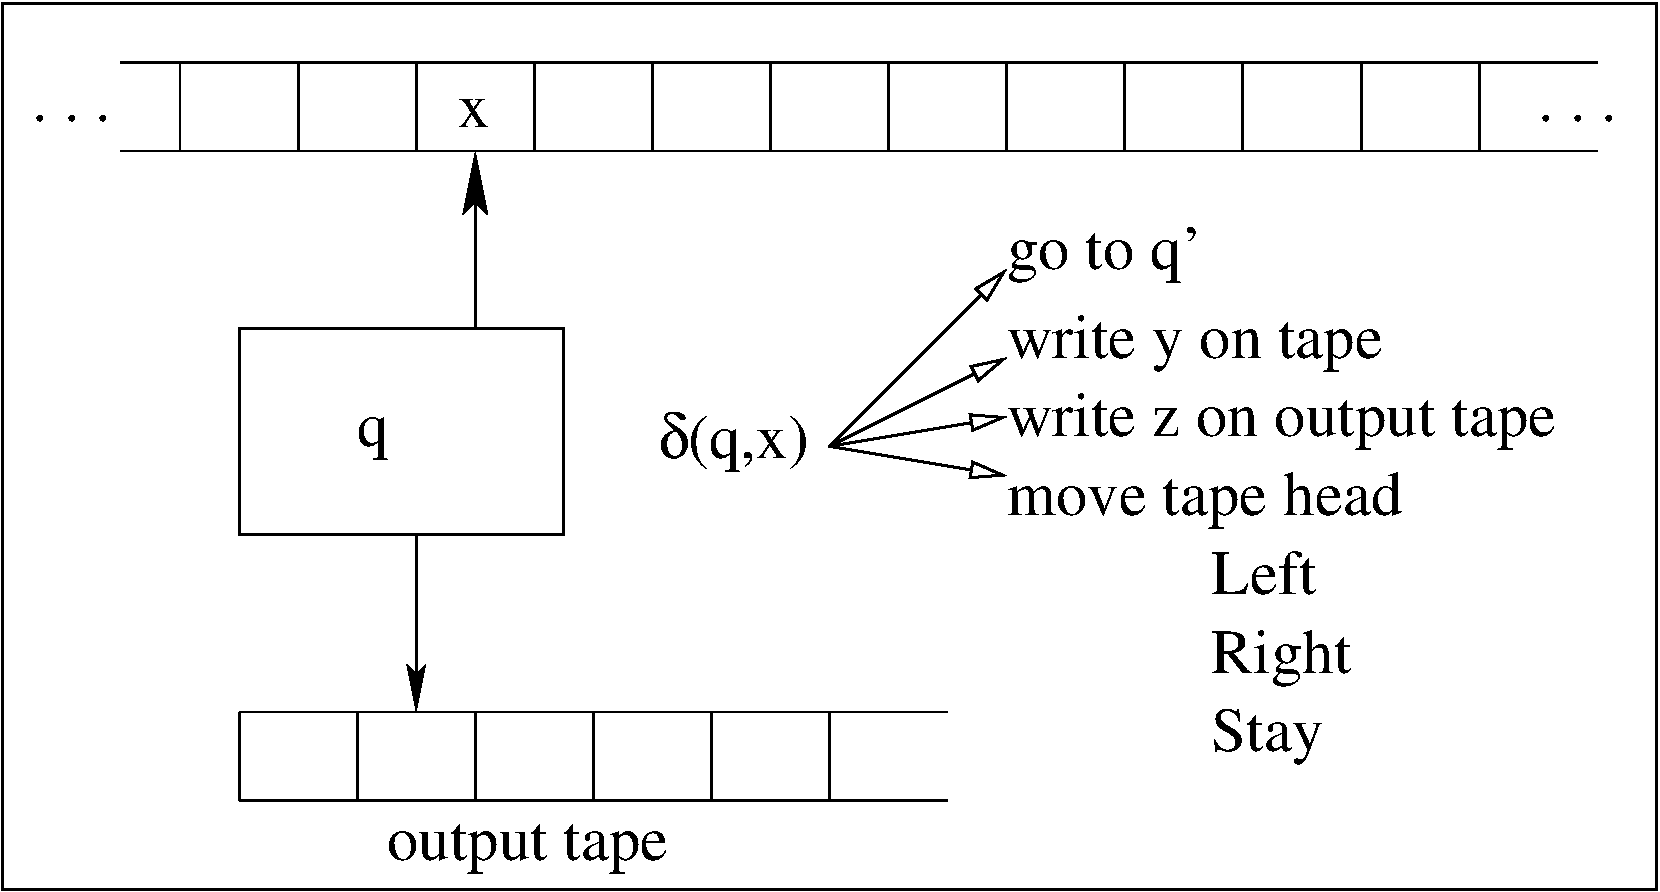
\includegraphics[%
  width=0.7\linewidth,
  keepaspectratio]{enumerator1eng}
\end{center}
\caption{Schema of an enumerator machine\label{enumerator1}}
\end{figure}

In Figure~\ref{enumerator1} you can see \marton{1 and 3 are not visible on the figure} that the enumerator is like a
Turing Machine with some extras
\begin{itemize}
\item an enumerator state $q_e$
\item an output tape
\item an output marker
\end{itemize}
The signature of its $\delta$ is
%
$Q \times \Gamma \rightarrow Q \times \Gamma \times \Gamma_\epsilon \times \{L,R,S\}$.
The last $\Gamma_\epsilon$ is meant to be the symbol written at that
transition to the output tape.


The machine starts with an empty tape and empty output tape, in the
usual $q_s$ and starts working. Whenever something is written on the
output tape, the write head moves one position to the right. Whenever
the machine gets in state $q_e$, the output marker is written on the
output, the machine goes to state $q_s$ and the machine continues.

It is possible that the enumerator does not stop, and outputs one
after another from a set of strings (separated by output markers):
this set could be finite, or infinite (can it be uncountably
infinite?). It is possible that the enumerator does not stop, and
keeps working on a particular output string, maybe even the first one!
It is also possible that the machine stops after a while and leaves a (finite!) set of strings on
the output separated by output markers.

Whichever of the above scenarios, it makes sense to talk about the set
of (finite) output strings produced by the enumerator: that is the
language determined by the enumerator, or enumerated by the
enumerator. The enumerator is allowed to produce the same output
string multiple times. We can now prove:

\begin{theorem}
The language enumerated by an enumerator is recognizable, and every
recognizable language can be enumerated by an enumerator.
\end{theorem}
\begin{proof}
(1) Given an enumerator Enu for L, we describe informally a recognizer
  M for L: M uses Enu as a subroutine as follows:
\begin{itemize}
\item[]
On input s, M starts Enu. Any time Enu is in its $q_e$ state, M
inspects the most recently produced string on the output tape of
Enu. If it equals s, M accepts s. Otherwise Enu continues.
\end{itemize}

(2) Suppose M recognizes L. We construct an enumerator Enu for L with the following ingredients:

\begin{itemize}
\item[-]
a $TM_{gen}$ that given a number $n$ puts the first $n$
strings from $\Sigma^*$ on a tape: $s_1, s_2, ... s_n$

\item[-]
a $TM_n$ that executes $n$ transitions
of M on each of the $n$ strings: if a string $s_i$ is accepted within that budget, it is written
on the output tape of Enu

\item[-]
a $TM_{driver}$ that generates the numbers 1,2,... one after the
other and for each of them calls $TM_{gen}$ and $TM_n$

\end{itemize}
\end{proof}

Why did we need acquaintance with the halting problem? Naively, we
would have proposed the following procedure to make an enumerator Enu
out of a Turing Machine TM:

\begin{itemize}
\item[]
generate the strings from $\Sigma^*$ in any order:
$s_1, s_2...$

\item[]
give each $s_i$ as input to M and if M accepts, output $s_i$
\end{itemize}

That does not work, because M might loop on some $s_i$, and thanks to
the halting problem, we understand there is no way to know this in
advance. Suppose $s_{i+1}$ belongs to $L_M$, then our thus constructed
Enu would not enumerate it.


% \clearpage
\section{Decidable languages}

\subsection{Related to regular languages}

The sentence {\em regular languages are decidable} might be ambiguous:
we must specify precisely what is input to the decider. So we refine
that sentence, depending on how the regular language itself is given.


\begin{itemize}
\item
$A_{DFA} = \{\langle D,s \rangle|D~is~a~DFA,~and~D~accepts~s\}$
\item
$A_{NFA} = \{\langle N,s \rangle|N~is~a~NFA,~and~N~accepts~s\}$
\item
$A_{RegExp} = \{\langle RE,s
  \rangle|RE~is~a~regular~expression,~and~RE~generates~s\}$
\end{itemize}

\begin{theorem} \label{reglandec}
$A_{DFA}$, $A_{NFA}$ and $A_{RegExp}$ are decidable.
\end{theorem}
\begin{proof}
The proof is constructive.
\begin{itemize}
\item
The decider B has input $\langle D,s \rangle$. B simulates D on s. If
D accepts s, B stops in its $q_a$. If D rejects s, B stops in its
$q_r$. Looping does not occur.

\item
The simulation of an NFA can loop, unless one performs loop detection
... We chose an easier path: the decider B has input $\langle D,s
\rangle$. B transforms the NFA D to a DFA (see the algorithm in
Section~\ref{detfsa}). Now use the above simulation.

\item
Given input $\langle RE,s \rangle$, first transform the RE to an NFA
and proceed as above.
\end{itemize}
\end{proof}

The technicalities of reductions are introduced only later, but
above, we used the principle of reduction twice.

We can also prove that any regular language is decidable. Try to
understand the subtle difference with the statement in
Theorem~\ref{reglandec}. (there is a hint in the proof)

% \clearpage
The following three questions about a language are quite popular:
\begin{itemize}
\item does the language contain the empty string?
\item is the language empty?
\item are two given languages equal?
\end{itemize}

Pertaining to regular languages, we can construct a decider for each
of these questions, but once more, we need to specify what is the
input to the decider. Instead of constructing the decider as a TM, we
will informally explain its working. Make sure that all steps are
realizable as a TM.


The first question is trivial, because $A_{DFA}$ is decidable.

\begin{theorem}
$E_{DFA} = \{\langle DFA \rangle| L_{DFA} = \phi\}$ is decidable.
\end{theorem}
\begin{proof}
There are many ways to prove this. Here is one that uses some theory
we studied before, but is also a bit of an overkill: you are invited
to find shorter and/or more elegant ways.

Transform the DFA to a minimal $DFA_{min}$ accepting the same language.
If $L_{DFA} = \phi$ then $DFA_{min}$ is isomorphic with ... (draw that
machine). Deciding that is easy.
\end{proof}

\begin{theorem}
$EQ_{DFA} = \{\langle DFA_1,DFA_2 \rangle| L_{DFA_1} = L_{DFA_2}\}$ is decidable.
\end{theorem}
\begin{proof}
We use some algebraic properties of the set of DFAs.

From $DFA_1$ and $DFA_2$, construct $DFA_\Delta$ that accepts the
symmetric difference between $L_{DFA_1}$ and $L_{DFA_2}$. Then decide
whether $DFA_\Delta$ accepts the empty language using the previous
theorem. (did you see the reduction?)
\end{proof}


\paragraph{Selfie:} Find other proofs for the theorems above.

% \clearpage
\subsection{Related to context free languages}

The questions are similar to the ones in the previous section, and can
be formulated either by giving the CFG or the PDA for the context free
language at hand. We show it for the grammar only.

\begin{theorem} \label{acfg}
$A_{CFG} = \{\langle G,s \rangle|G~is~a~CFG,~and~s \in L_G\}$ is
    decidable: {\em acceptance} of a string by a CFG is decidable.
\end{theorem}
\begin{proof}
A naive proof idea consists in using the CFG to generate strings, and
accepting as soon as s is generated. You can see why this does not work:
when do you reject? We have a recognizer, not a decider.

It would be convenient if the CFG were in Chomsky Normal Form: we
would then have an upper bound on the length of the derivation for a
given string.

So, for input $\langle G,s \rangle$, first convert G to its Chomsky
Normal Form. Generate all possible strings with a derivation length
$2|s|-1$: there are only finitely many of them. If s is one of them,
accept, otherwise reject.
\end{proof}

\begin{theorem}
$E_{CFG} = \{\langle G \rangle|G~is~a~CFG,~and~L_G = \phi\}$ is decidable: {\em emptiness} of a CFL is decidable.
\end{theorem}
\begin{proof}
We informally describe an algorithm transforming G to a form in which
taking the decision is easier.
\begin{itemize}
\item
for a rule $A \rightarrow \alpha$ with $\alpha$ only terminal symbols
\begin{itemize}
\item remove all rules with A at the left side
\item replace the occurrences of A in any right side by $\alpha$
\end{itemize}


\item
keep doing this until
\begin{itemize}
\item the start symbol is removed: reject, because the start symbol
  can derive a string
\item there are no rules of the required form: accept, because the
  language is empty
\end{itemize}
\end{itemize}
\end{proof}

Be careful with the above proof: the grammar is transformed to a
non-equivalent one!


\paragraph{Selfie:}
Write down a grammar that determines the empty language and apply the
above procedure to it. Did you learn something about Prolog programs
that have no answers?

\begin{theorem} \label{escfg}
$ES_{CFG} = \{\langle G \rangle|G~is~a~CFG,~and~\epsilon \in L_G\}$ is
    decidable: it is decidable whether a CFG generates the empty string.
\end{theorem}
\begin{proof}
Transform the CFG to its Chomsky Normal Form. If it now contains the
rule $S \rightarrow \epsilon$, accept, otherwise reject.
\end{proof}

\begin{theorem}
Every CFL is decidable.
\end{theorem}
\begin{proof}
Here, the question is to prove the existence of a decider $B_G$ that
can decide for each string whether it belongs to G or not. Appreciate
the difference with $A_{CFG}$. Work out the details yourself.
\end{proof}

The remaining one is $EQ_{CFG}$, i.e. if we get two CFGs, can we
decide whether they have the same language? The decider for $EQ_{DFA}$
relied on the symmetric difference of regular languages. We can not
use the same idea for CFLs, because they are not closed under
complement or intersection.

\paragraph{Selfie:}
\begin{itemize}
\item[]
Prove that $\overline{EQ_{CFG}}$ is recognizable.

What does that mean for $EQ_{CFG}$?

Prove that Theorem~\ref{escfg} follows directly from Theorem~\ref{acfg}.
\end{itemize}

% los eindje in de cursus: nergens wordt bewezen dat $EQ_{CFG}$
% niet-recognizable is


% \clearpage
\section{Undecidable languages}

In Section~\ref{halting} we proved that $A_{TM}$ and $H_{TM}$ are not
decidable. Here are some more of the same kind.

\begin{theorem} \label{nonreductie1}
$E_{TM} = \{\langle M \rangle | M~is~a~TM,~and~L_M = \phi\}$ is not
     decidable: it is not decidable whether a Turing Machine accepts
     no input.
\end{theorem}
\begin{proof}
Assume that $E_{TM}$ is decidable, then there exists a decider $E$ for
it. We now describe a decider B for $A_{TM}$ using $E$:
B receives as input $\langle M,s \rangle$ and works as follows:
\begin{itemize}
\item
it constructs a machine $M_{M,s}$ whose working is given by: on input
$w$, $M_s$ does the following
\begin{itemize}
\item if $w \neq s$, reject
\item else run M on $w$ (or $s$) and return the same result
\end{itemize}

\item
run $E$ on input $\langle M_{M,s} \rangle$
\begin{itemize}
\item if $E$ accepts $\langle M_{M,s} \rangle$, then B rejects its
  input $\langle M,s \rangle$; indeed: $M_{M,s}$ determines the empty
  language, so M has not accepted s
\item if $E$ rejects $\langle M_{M,s} \rangle$, B accepts its input: since  $M_{M,s}$ is not empty, M accepts s
\end{itemize}

\end{itemize}
It follows that B is a decider for $A_{TM}$, which is impossible, so
$E$ does not exist, so $E_{TM}$ is not decidable.
\end{proof}

We can define the $E_{TM}$ problem slightly differently, as an instance
of a more general problem: does a given machine M determine a language
from a given set? So we have

$~~~~~~~~~IsIn_{TM,S} = \{\langle M \rangle| L_M \in S\}$.


Then $E_{TM} = IsIn_{TM,\{\phi\}}$


Another instance of the general problem:
\begin{itemize}
\item[] does a given Turing Machine M determine a regular language,
  i.e.  is $IsIn_{TM,RegLan}$ decidable? We denote that problem as
$REGULAR_{TM}$
\end{itemize}

\begin{theorem}
$REGULAR_{TM}$ is not decidable.
\end{theorem}
\begin{proof}
Suppose Turing Machine $R$ decides $REGULAR_{TM}$. Fix two symbols
from the alphabet, say 0 and 1. Make a decider $B$ for $A_{TM}$ as
follows: on input $\langle M,s \rangle$ $B$ does the following:
\begin{itemize}
\item it constructs a helper machine $H_{M,s}$ that on input $x$ does
  the following
\begin{itemize}
\item if $x$ is of the form $0^n1^n$, accept
\item else let $M$ run on $s$; return the same answer
\end{itemize}

\item then $B$ lets $R$ run on  $\langle H_{M,s} \rangle$
\item if $R$ accepts, accept; if $R$ rejects, reject
\end{itemize}

First note that $H_{M,s}$ never runs: it is there only as input for
$R$. Finishing the proof:


$H_{M.s}$ either accepts the non-regular language $\{0^n1^n\}$
or the regular language $\Sigma^*$. So, $B$ accepts $\langle
M,s \rangle$ iff $R$ accepts $\langle H_{M,s} \rangle$, iff $H_{M,s}$
accepts $\Sigma^*$, iff $M$ accepts $s$. It follows that $B$ is a
decider for $A_{TM}$, which is impossible, so $R$ does not exist, so
$REGULAR_{TM}$ is not decidable.
\end{proof}

\begin{theorem} \label{reduction1}
$EQ_{TM}$ is not decidable.
\end{theorem}
\begin{proof}
We already know that $E_{TM}$ is not decidable. $E_{TM}$ is a special
case of $EQ_{TM}$, in which the second machine is $M_\phi$. It is
clear that if we could decide the equality of two arbitrary languages,
we would also be able to decide about one arbitrary language
and the empty one. So, we arrive at a contradiction by assuming that
$EQ_{TM}$ is decidable.
\end{proof}

The above proof technique is studied in more detail in
Section~\ref{mappingreduction}.

% \clearpage

The following is about context sensitive languages. We first define
the machinery needed to decide them:

\begin{definition}[Linear Bounded Automaton]
A Linear Bounded Automaton is a (non-deterministic) Turing Machine
that reads and writes only on the part of the tape that contained the
initial input.
\end{definition}

The name of the automaton might strike you as weird. An equivalent
definition allows the machine to use a portion of the tape that is
larger by a constant factor $f$ than the input: this $f$ is
independent of the input. We mentioned earlier that such machines can
decide context sensitive languages. You can intuitively work that out
by adhering to the alternative definition of context sensitive grammar
on page \pageref{altdefcs}, trying out a bottom-up parse, and notice
that you do not need extra space.

There is no decision procedure for deciding whether a given Turing
Machine is actually an LBA (adapt the proof for $REGULAR_{TM}$). But a
TM can be turned into an LBA by adding a marker at the left and right
of the input, and adapting the transition table so that this marker is
never crossed.\footnote{{\bf Selfie}: show with an example that in
  general you have changed the language!}


The acceptance problem for LBAs is

$~~~~~~~~~A_{LBA} = \{\langle M,s \rangle | M~is~an~LBA~and~s \in L_{LBA}\}$.

The following might surprise you ...

\begin{theorem}
$A_{LBA}$ is decidable.
\end{theorem}
\begin{proof}
Consider the configurations that can occur during the execution of
an LBA on an input with length $n$. Using $q$ for the number of states
of the LBA, and $b$ for the size of the tape alphabet, we can quickly
compute the number of possible tape contents: it is bounded by
$b^n$. The tape head can be on any cell of the allowed portion of the
tape, so the upper bound for the number of configurations is $qnb^n$.

A decider B for $A_{LBA}$ can now be constructed as follows:
on input $\langle M,s \rangle$, B performs the following
\begin{itemize}
\item it computes $Max = qnb^n$
\item it simulates $M$ on $s$ for at most $Max$ steps
\item if $M$ accepted in the mean time, accept
\item if $M$ rejected in the mean time, reject
\item if $M$ has not yet stopped, it means that $M$ loops and does not
  accept: reject
\end{itemize}
\end{proof}

\begin{theorem}
$E_{LBA} = \{M | M~is~an~LBA~with~L_M = \emptyset\}$ is not decidable.
\end{theorem}
\begin{proof}
We first show that for a given Turing Machine $M$ and string
$s$, we can construct an LBA that can decide about a finite sequence
of configurations of $M$, whether it is an accepting computation
history for $s$. A sequence of configurations can be put on a tape
easily as in the figure below
\begin{center}
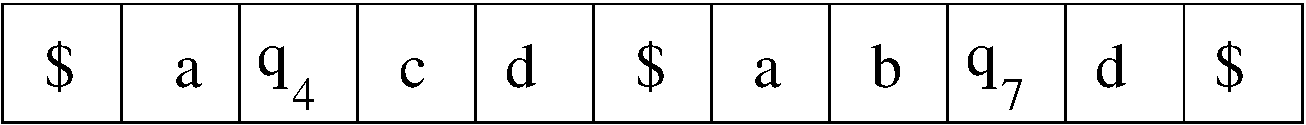
\includegraphics[%
  width=0.5\linewidth,
  keepaspectratio]{comphistband}
\end{center}
It represents a transition for which $\delta(q_4,c) = (q_7,b,R)$.

To check whether a sequence of configurations is an accepting computation
history for $s$, the following is needed:
\begin{itemize}
\item check that two subsequent configurations are connected through
$\delta$
\item check that the first configuration is of the form $q_ss$
\item check that the last configuration contains $q_a$
\end{itemize}

It should be clear - at least intuitively - that these checks need at
most a constant amount of extra space, meaning that the decision can
be taken by an LBA. We construct the LBA in such a way that it accepts
the accepting computation history for $s$, and rejects every other
input.  We can now start the proof.

Suppose we have a decider $E$ for $E_{LBA}$. We construct a decider
$B$ for $A_{TM}$ as follows. On input $\langle M,s \rangle$ $B$
performs the following actions:
\begin{itemize}
\item it constructs the LBA $A_{M,s}$ as above described: this LBA can
  decide whether a given string is an accepting computation history
  for $M$ on input $s$
\item give $\langle A_{M,s} \rangle$ to $E$: if $E$ accepts, reject;
otherwise accept
\end{itemize}
$B$ decides $A_{TM}$ because $B$ accepts $\langle M,s \rangle$ iff $E$
rejects $\langle A_{M,s} \rangle$, iff $A_{M,s}$ accepts at least one
string, iff there exists an accepting computation history for $M$ on
$s$. The latter is equivalent with $M$ accepts $s$.

So, $B$ does not exist, so neither can $E$, and as a conclusion:
$E_{LBA}$ is not decidable.
\end{proof}

A small summary of the differences and similarities between PDAs, LBAs
and TMs follows:

\begin{itemize}
\item acceptance and halting
\begin{itemize}
\item PDA and LBA are similar: acceptance and halting are decidable
\item TM is different: acceptance and halting are not decidable
\end{itemize}
\item emptiness
\begin{itemize}
\item LBA are TM are similar: emptiness is not decidable
\item PDA differs: emptiness is decidable
\end{itemize}
\end{itemize}

To conclude for now: it is not decidable whether a CFG generates all
strings from $\Sigma^*$, i.e. $ALL_{CFG} = \{\langle G \rangle|L_G =
\Sigma^*\}$ is not decidable. That is a bit weird, as $E_{CFG}$ is
decidable. Then again, complement is not internal for CFLs ...

\begin{theorem}
$ALL_{CFG}$ is not decidable.
\end{theorem}
\begin{proof}
No proof this year.
\end{proof}

\paragraph{Selfie:} Prove that $ALL_{RegExp}$ is decidable.

% \clearpage
\section{Some trivia on languages}

Let $Dec$ denote the set of decidable languages, and $Rec$ the
recognizable languages. First some inclusions, all strict:

\begin{itemize}
\item[] $RegLan \subset DCFL \subset CFL \subset Dec \subset Rec
\subset {\cal P}(\Sigma^*)$
\end{itemize}

Some properties of operations on languages:

\begin{itemize}
\item[] $RegLan$ is closed under union, intersection and complement
\item[] $DCFL$ is closed under complement, but $CFL$ is not
\item[] $CFL$ is closed under union, but $DCFL$ is not
\item[] $Dec$ is closed under union and complement
\item[] $Rec$ is closed under union
\end{itemize}

Let us also have a look at a somewhat unusual operation on languages:
inversion. Denote the string obtained by writing the
symbols of $s$ in reverse order with $\hat{s}$. We define $\widehat{L} = \{\hat{s}|s
\in L\}$.

\begin{itemize}
\item[] $RegLan$, $CFL$, $Dec$ and $Rec$ are closed under inversion
\item[] $DCFL$ is NOT closed under inversion
\end{itemize}

{\bf Example:} The language
%
$L = \{ba^mb^nc^k|m \neq n\} \cup \{ca^mb^nc^k|n \neq k\}$ is
deterministic context free (construct its DCFG) but $\widehat{L}$ is
not.


% \clearpage
\section{Countable}

A set $V$ is countable if there exists a bijection between $V$ and (a
part of) $\N$. This definition is about {\em existence} and it does
not care about the ease with which the bijection can be computed: as
far as the definition goes, there is no need for that.

Still, in the context of computability, we care about such bijection
being computable by a Turing Machine. We have indeed used
constructions that use a TM that generates the strings of $\Sigma^*$
one by one. It is thus not enough that $\Sigma^*$ is countable, it
needs to be (effectively) enumerable (by a TM). You should be able to prove at
this point that there exist subsets of $\Sigma^*$ that are
not enumerable, and give concrete examples as well.

So, what is the connection between being generated by an enumerator
machine, and effectively enumerable? The enumerator is allowed to
generate duplicates. We can prevent it from doing so by modifying it a
little: any time the enumerator arrives in its enumerator state, we
check whether the most recently generated string is really new: if
not, we erase it. Now the enumerator effectively enumerates all its
strings. Since every language generated by an enumerator is recognizable,
and since we proved that there exists a non-recognizable language L,
it follows that this L can not be enumerated, although it is
countable.

\paragraph{Selfie:} Construct languages that are countable, but not enumerable.

% \clearpage
\section{How to kill $N$ birds with one stone: Rice's Theorem}

We have seen some concrete examples of undecidable languages, often by
reduction to $A_{TM}$: every time, we found a new little trick so that
a supposed decider for a language could be used in a decider for
$A_{TM}$ and lead to contradiction. So, Rice's theorem comes as a
relief: in one go, it proves that a whole lot (how many?) languages
are undecidable.

Consider the set of Turing Machines (for convenience over a fixed
alphabet). A property $P$ of the Turing Machines splits the set in two
parts: the machines that have property $P$, denoted
%
$Pos_P = \{M|P(M) = true\}$, and the machines that do not have the
property, denoted
%
$Neg_P = \{M|P(M) = false\}$.

\begin{definition}[Non-trivial property]
A property $P$ of TMs is {\em non-trivial} if

$~~~~~~~~~~~~Pos_P \neq \emptyset$ and also $Neg_P \neq \emptyset$.
\end{definition}

\begin{definition}[Semantic property]
The property $P$ is {\em semantic} if

$~~~~~~~~~L_{M_1} = L_{M_2} \Longrightarrow P(M_1) = P(M_2)$

or in words: {\em machines recognizing the same language either all
  have $P$ or none have $P$}.
\end{definition}

\paragraph{Selfie:}
\begin{itemize}
\item[]
Invent some examples of semantic, non-trivial
properties of TMs.

Invent some examples of properties of TMs that are not semantic.

For a given non-trivial and semantic property $P$, how many
machines have $P$? How many don't?
\end{itemize}

% \clearpage

\begin{theorem}[Theorem I by Rice]
Let $P$ be a non-trivial, semantic property of Turing
Machines. $Pos_P$ (and $Neg_P$) is undecidable.
\end{theorem}
\begin{proof}
Suppose $M_\emptyset$ (a machine deciding the empty language) does not
have property $P$ - if not, replace $P$ by its negation. Since $P$ is
non-trivial, there also exists a machine $X$ having $P$ - denote
its language by $L_X$. Suppose $Pos_P$ were decidable by a decider
$B$. We will use $B$ to construct a decider $A$ for $A_{TM}$.

$A$ has as input $\langle M,s \rangle$ and does the following:
\begin{itemize}
\item construct a helper machine $H_{M,s}$ that on input $x$:

\begin{itemize}
\item runs $M$ on $s$
\item if $M$ accepts $s$, lets $X$ run on $x$ and returns its result
\end{itemize}

\item now give $H_{M,s}$ to $B$
\item if $B$ accepts $H_{M,s}$, accept, else reject
\end{itemize}
First check that $H_{M,s}$ accepts either the empty language or
$L_X$. This is used in the following:


$A$ accepts $\langle M,s \rangle$ iff $B$ accepts $H_{M,s}$, iff
%
$H_{M,s}$ has property $P$, iff
%
$H_{M,s}$ accepts $L_X$, iff
%
$M$ accepts $s$.

So, $A$ is a decider for $A_{TM}$, clearly impossible, so $B$ does not
exist, and $Pos_P$ is not decidable.
\end{proof}

Rice also has a second theorem: every non-monotone property is not
recognizable; it is worth having a look at it!

\paragraph{Selfie:}
\begin{itemize}
\item[]
What can you conclude regarding whether $Pos_P$ and/or $Neg_P$ are
recognizable?

Use Rice for new proofs of old theorems.
\end{itemize}


\clearpage
\section{The {\em Post Correspondence Problem}}

Emil Post was one of the founding fathers of recursion theory, and he
made contributions to universal computing mechanisms. The word {\em
  correspondence} is related to {\em similarity, agreement}, not to
sending mail by post. Emil Post developed the following game:

You have a finite collection of dominoes, each with two strings
(instead of the usual numbers). Of each type, there is an unlimited
supply for this game. If you put some dominoes next to each other, you
see an upper string and a lower string. The question is: is it
possible to lay out a finite number of dominoes so that the upper and
lower strings are the same?

An example:
\begin{figure}[h]
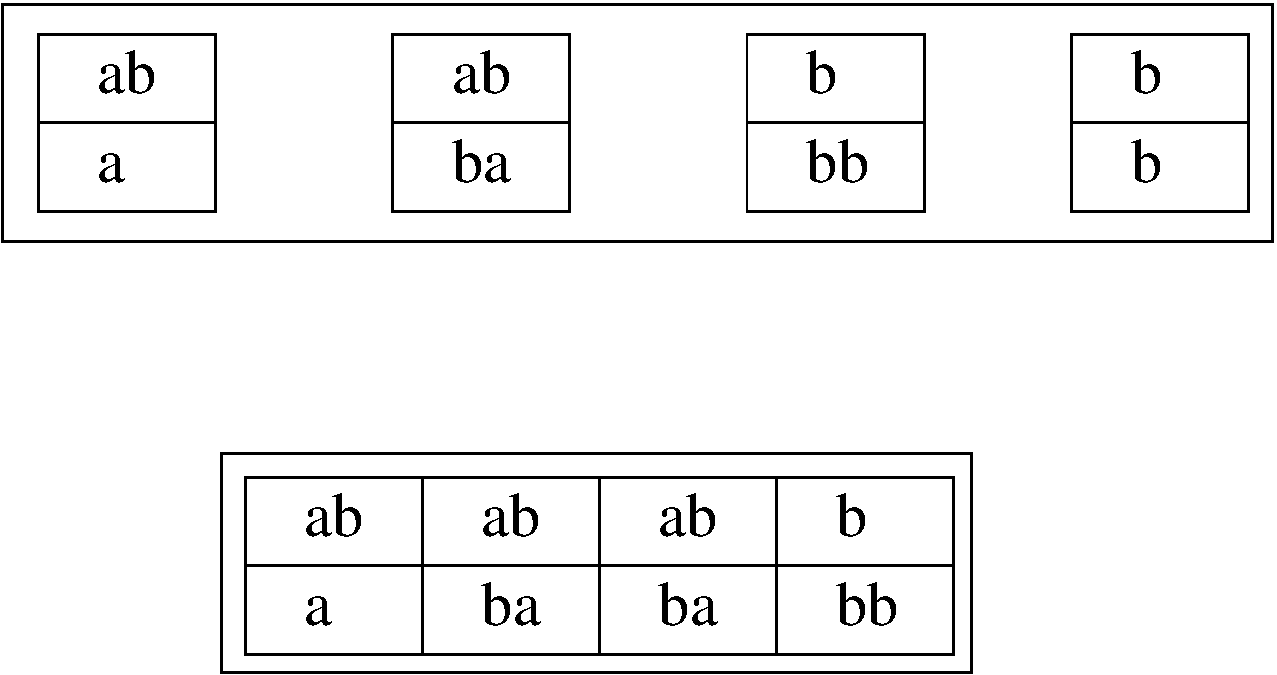
\includegraphics[%
  width=0.5\linewidth,
  keepaspectratio]{pcp1}
\caption{Four given dominoes and a solution\label{pcp1}}
\end{figure}

\vspace{-5cm}\hspace{10cm}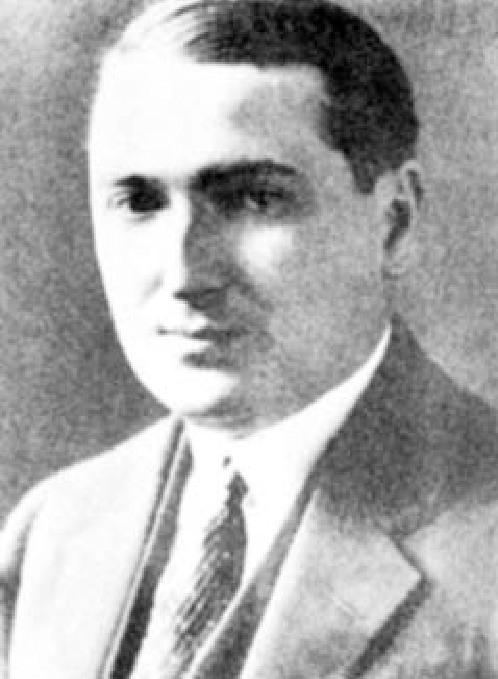
\includegraphics[%
  width=0.2\linewidth,
  keepaspectratio]{static/post}




\vspace{0.5cm}
Figure~\ref{pcp1} shows that you don't need to use all dominoes and
that one type of domino can be used more than once.

We are dealing here with a decision problem: it is enough to answer
yes or no to the question, there is no need to construct the
corresponding sequence of dominoes.

This simple game is (1) undecidable and (2) powerful enough to mimic all
computations by all Turing Machines. Actually, the former follows from
the latter, as soon as we have shown that the halting of a TM can be
reduced to the existence of a solution to the PCP. We show this by
example: the books by Sipser or Minsky contain a general construction.

\subsection{Turning a Turing Machine into a PCP game}

In this example we use X for the start state, A for the accepting
state, Z for the reject state. The alphabet is $\{a,b\}$, and the
transition table looks like:

\begin{center}
\begin{tabular}{|r||l|l||l|l|l|}
\hline
1 & X & a & B & a & R \\
2 & X & b & Z & \_ & \_ \\
3 & X & \# & A & \# & S \\
4 & B & a  & Z & \_ & \_ \\
5 & B & b  & X & b  & R  \\
6 & B & \# & Z & \_ & \_ \\
\hline
\end{tabular}
\end{center}

The numbers at the left are there for ease of reference. Check that
this TM accepts the language $(ab)^*$. Take $ab$ as the input string.
%
We introduce an extra symbol \$. We now define the dominoes needed in
the Post game for imitating the above Turing Machine:

\begin{itemize}
\item for each symbol $x$ create a domino with both the upper and lower string
  equal to $x$, i.e. 4 dominoes:
\begin{tabular}{|l||l||l||l|}
\hline
a & b & \$ & \# \\ \hline
a & b & \$ & \# \\
\hline
\end{tabular}
and dominoes with Ax or xA as the upper string, and A as lower
string, i.e. 8 dominoes:
\begin{tabular}{|l||l||l||l|}
\hline
aA & bA & \$A & \#A \\ \hline
A & A & A & A \\
\hline
\end{tabular}
\begin{tabular}{|l||l||l||l|}
\hline
Aa & Ab & A\$ & A\# \\ \hline
A & A & A & A \\
\hline
\end{tabular}

\item rule 1 in the transition table results in a domino
\begin{tabular}{|l|}
\hline
Xa \\ \hline
aB \\
\hline
\end{tabular}

\item from rule 5 we get
\begin{tabular}{|l|}
\hline
Bb \\ \hline
bX \\
\hline
\end{tabular}

\item
from rule 3
\begin{tabular}{|l|}
\hline
X\# \\ \hline
A\# \\
\hline
\end{tabular}


\item
the following dominoes do not depend on the TM

the end domino
\begin{tabular}{|l|}
\hline
A\$\$                     \\ \hline
   \$                     \\
\hline
\end{tabular}
and the blank generators left and right
\begin{tabular}{|l||l|}
\hline
        \$   & \$         \\ \hline
        \$\# & \#\$       \\
\hline
\end{tabular}

\item
finally, the input $ab$ turns into a starting domino
\begin{tabular}{|l|}
\hline
\$ \\ \hline
\$Xab\$ \\
\hline
\end{tabular}
\end{itemize}

The question is now: construct a correspondence with these dominoes,
starting from the input domino.\footnote{The general PCP allows to
  start from an arbitrary domino: one problem can be reduced to the
  other.} Here is the solution:


% \hspace{-1.5cm}
{\footnotesize
\begin{tabular}{|l|l|l|l|l|l|l|l|l|l|l|l|l|l|l|l|l|l|l|l|l|l|l|l|l|l|l|l|l|l|l|l|l|l|}
\hline
\$      & Xa & b & \$   & a & Bb & \# & \$ & a & b & X\# & \$ &  a & bA & \# & \$ & aA & \# & \$ & A\# & \$ & A\$\$\\ \hline
\$Xab\$ & aB & b & \#\$ & a & bX & \# & \$ & a & b & A\# & \$ &  a &  A & \# & \$ & A  & \# & \$ & A   & \$ & \$  \\
\hline
\end{tabular}
}


In the lower half, you see a configuration between any two occurrences of \$;
two subsequent configurations are linked by the
transition function until the accepting state appears. After that,
the configuration is emptied until only the accepting state and the
end domino appears. Now, upper and lower are equal.


\paragraph{Selfie:}
\begin{itemize}
\item[]
Convince yourself that by starting with an input string not in the
language $(ab)^*$, no correspondence can be found.

Find out about the general correspondence between $\delta$ and the
dominoes: our $\delta$ did not have movements to the left!

Formulate more precisely the link between PCP and $H_{TM}$.
\end{itemize}



% \clearpage
\paragraph{An extra: the Post tag machine}

E. Post is also known for his {\em tag systems} or {\em Post tag
  machines}. Just a small example of a 2-tag system:

\begin{itemize}
\item the alphabet is $\{a,b,c\}$ and there is also a halt symbol H
\item the rules are
\begin{itemize}
\item a \rpijl aa
\item b \rpijl accH
\item c \rpijl a
\end{itemize}

\item the initial word is aab
\item and here is a derivation starting from the initial word

aab \rpijl baa \rpijl aaccH \rpijl ccHaa \rpijl Haaa
\end{itemize}

The general rule for rewriting is: the first letter of the word
decides which rule is used (this could be the source of
non-determinism). Now add the right side of such a rule at the end of
the string, and erase 2 symbols at the front (the same 2 as in 2-tag
system).

The derivation ends when H appears at the front of the string: the
rest of the string can be considered the result of a computation
starting with the initial string.

This rewriting system is also Turing complete.


2-tag systems have been used to simulate small UTMs.


\clearpage
\section{Many-one reduction}\label{mappingreduction}

A reduction maps one problem L1 to another L2: it seems a bit counterintuitive,
but L2 is in some sense {\em more difficult} than L1,
because a method to solve L2 is (together with the reduction) powerful
enough to solve L1. We will make all this very precise. It is important
to get a good grasp on the reductions in this section: in complexity
theory, we use similar reductions, so it is a recurring concept.

%

\begin{definition}[(Turing) computable function]
A function $f$ is (Turing)
       computable if there exists a Turing Machine that on input $s$
       eventually halts with $f(s)$ on the tape.
\end{definition}

We do not care whether the machine stops in an accepting or a
rejecting end state.

\begin{definition}[Many-one Reduction of languages] \label{manyone}
A many-one reduction of language $L_1$ (over $\Sigma_1$) to language
$L_2$ (over $\Sigma_2$) is a total computable function $f$ from
$\Sigma_1^*$ to $\Sigma_2^*$ so that $f(L_1) \subseteq L_2$ and
%
$f(\overline{L_1}) \subseteq \overline{L_2}$.

We denote this by $L_1 \leq_m L_2$, and we can also say {\em $L_1$
  reduces to $L_2$}, or {\em $L_1$ is mapping reducible to $L_2$}.
\end{definition}

Figure~\ref{mapred} shows the condition on $f$.
% \clearpage
\begin{figure}[h]
\begin{center}
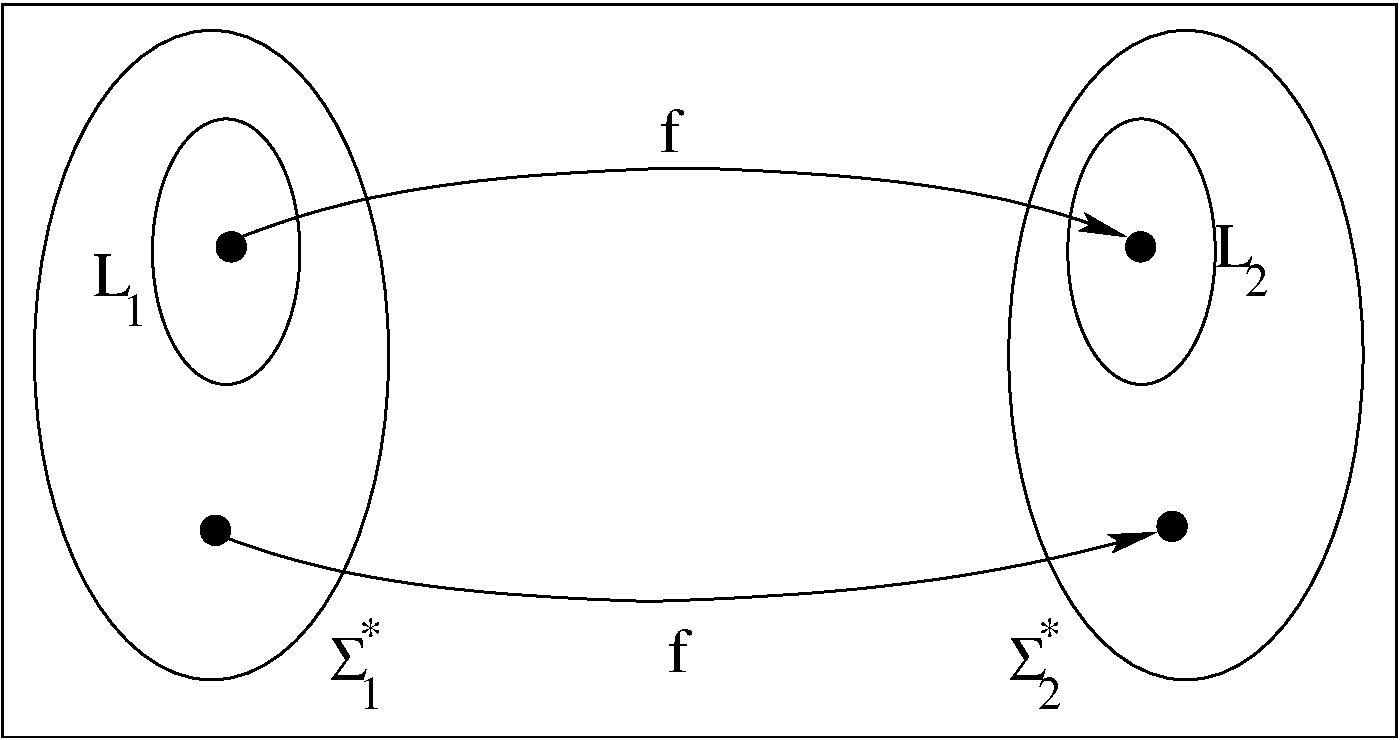
\includegraphics[%
  width=0.6\linewidth,
  keepaspectratio]{mapred}
\end{center}
\caption{Schematic representation of a reduction\label{mapred}}
\end{figure}

A reduction $f$ offers a method to transform the decision question
about $L_1$ into a decision question about $L_2$, indeed,
%
$s \in L_1?$ can be answered by deciding about $f(s) \in L_2$. The
next theorems make that more precise: you must be able to prove them.

\begin{theorem}
If $L_1 \leq_m L_2$ and $L_2$ is decidable, then $L_1$ is decidable.
\end{theorem}

\begin{theorem}
If $L_1 \leq_m L_2$ and $L_2$ is recognizable, then $L_1$ is recognizable.
\end{theorem}

\begin{corollary}
If $L_1 \leq_m L_2$ and $L_1$ is not recognizable, then $L_2$ is not
recognizable.  If $L_1 \leq_m L_2$ and $L_1$ is not decidable, then
$L_2$ is not decidable.
\end{corollary}

We have used reductions informally in previous theorems, e.g. on page
\pageref{reduction1} when we proved that $EQ_{TM}$ is not decidable.
Let's do it now based on the definitions.

\begin{theorem}
$EQ_{TM}$ is not decidable.
\end{theorem}
\begin{proof}
We reduce $E_{TM}$ to $EQ_{TM}$: $f$ maps input $\langle M \rangle$ to
$\langle M,M_\phi \rangle$; $M_\phi$ a Turing Machine accepting the
empty language. Clearly, $f$ is Turing computable.

So, $E_{TM} \leq_m EQ_{TM}$, and since we know already that $E_{TM}$
is not decidable, $EQ_{TM}$ is not decidable either.
\end{proof}

\begin{theorem}
If $A \leq_m B$ then  $\overline{A} \leq_m \overline{B}$.
\end{theorem}
\begin{proof}
Selfie!
\end{proof}


Also on page \pageref{nonreductie1}, we used a reduction from
$\overline{A_{TM}}$ to $E_{TM}$: we mapped $\langle M,s \rangle$ to
$\langle M_s \rangle$ ...  Note that a mapping reduction from
$A_{TM}$ to $E_{TM}$ does not exist - can you explain why?

\begin{theorem}
$EQ_{TM}$ is not recognizable and not co-recognizable.
\end{theorem}
\begin{proof}
We construct two mapping reductions: $A_{TM} \leq_m
\overline{EQ_{TM}}$ and $A_{TM} \leq_m EQ_{TM}$. Since
$\overline{A_{TM}}$ is not recognizable, the result follows.
\begin{enumerate}
\item $f$ maps $\langle M,s \rangle$ to $\langle M_s,M_\phi \rangle$;
  $M_s$ is a machine that accepts every string if M accepts s; clearly
  $f$ is computable; we should also prove the other conditions:
\begin{itemize}
\item if M accepts s, then the languages of $M_s$ and $M_\phi$ are
  different
\item if M does not accept s, then the languages of $M_s$ and $M_\phi$
  are equal
\end{itemize}

\item now, $f$ maps $\langle M,s \rangle$ to $\langle M_s,M_{\Sigma^*}
  \rangle$; $M_{\Sigma^*}$ is a machine accepting all strings; $M_s$
  is like before; checking the conditions on $f$ should be
straightforward.
\end{enumerate}
\end{proof}



% \clearpage

\section{Oracle machines and a hierarchy of decidability}

Suppose we had another way to decide $A_{TM}$ - not a TM of course -
would there be a way to use that power to decide everything? Let's
make the question a bit more concrete:
\begin{itemize}
\item since no TM can decide $A_{TM}$, we must name this device
  differently: it is an {\em oracle}; we get back to the
  implementation of an oracle later ...

\item a TM must be able to consult the oracle, i.e. the oracle for
  $A_{TM}$ can be called by a TM as a subroutine, with a string $s$ as
  input to the oracle; the oracle needs only a finite number of steps
  to give its decision (is $s \in A_{TM}$?) to the TM

\item in this way, we build a so called oracle machine $O^{A_{TM}}$:
  it is a TM that can ask questions to the oracle for $A_{TM}$
\end{itemize}

It is clear that we can make an $O^{A_{TM}}$ that decides $A_{TM}$:
give the input $\langle M,s \rangle$ to the oracle, and return its
answer. So, the set of oracle machines with oracle $A_{TM}$ is
strictly stronger than the set of Turing Machines. Here comes another
example:

\begin{theorem}
There exists an $O^{A_{TM}}$ that decides $E_{TM}$.
\end{theorem}
\begin{proof}
We construct $O^{A_{TM}}$ as follows: on input $\langle M \rangle$
$O^{A_{TM}}$ performs the following actions
\begin{itemize}
\item
it constructs a Turing Machine $P$ that on input $w$ performs the
following actions
\begin{itemize}
\item run $M$ on all strings of $\Sigma^*$ (*)\label{allestrings}
\item if $M$ accepts a string, accept
\end{itemize}

\item ask the oracle for $A_{TM}$ whether $\langle P,x \rangle \in
  A_{TM}$

\item if the oracle answers {\bf yes}, reject; otherwise accept
\end{itemize}
If $L_M \neq \emptyset$, then $P$ accepts every input, and for sure
also input $x$; so, the oracle answers {\bf yes} and $O^{A_{TM}}$ must
reject. Vice versa: if $L_M = \emptyset$, then $O^{A_{TM}}$
accepts. We conclude that $O^{A_{TM}}$ decides the language $E_{TM}$.
\end{proof}

The theorem proves that $E_{TM}$ is decidable relative to
$A_{TM}$. The relevant definition is:

\begin{definition}[Turing reducible]
A language $A$ is Turing reducible to language $B$, if $A$
is decidable relative to $B$, i.e. there exists an oracle machine
$O^B$ that decides $A$. We write this as $A \leq_T B$.
\end{definition}

The definition supports our intuition about what it means for one
language to be reducible to another:

\begin{theorem}
If $A \leq_T B$ and $B$ is decidable, then $A$ is decidable.
\end{theorem}

The previous and following theorems are at your mercy!

\begin{theorem}
If $A \leq_m B$ then also $A \leq_T B$.

In other words: $\leq_m$ is finer than $\leq_T$.
\end{theorem}

Time for a description of an oracle for any language $L$: each
string has a running number in the lexicographic order on strings
(shorter before longer, and alphabetic). That means that the language
can be represented as an infinite bitmap: bit $i$ is one, if the
$i^{th}$ string is in L, and otherwise zero. That bitmap could be on a
tape. When an oracle gets a membership question about $s$, it first
computes its corresponding number, and then looks up the right bit
... So, do oracles exist or not?

Another question: can the class of oracle machines with an oracle for
$A_{TM}$ decide all languages? Certainly not, as a cardinality
argument can show you! So there exists a language $X$ that is not
decidable with an oracle for $A_{TM}$. You can now repeat the argument
for the $X$ oracle ... and you soon note that there is an infinite
hierarchy of ever more difficult languages. As a sidenote: also
complexity theory has its oracle machines and a nice hierarchy. The
difference is: the particular complexity hierarchy would still
collapse in case it turns out that $NP = P$. Our compatibility
hierarchy however stands strong!

\paragraph{Selfie:} In the theorem on page \pageref{allestrings},
a statement is marked by a (*): how can we let M run on all strings?
There are infinitely many of them ...




\clearpage
\section{The computable functions and the  recursive functions}

We gave a definition of Turing computable function in the previous
section. It was rather abstract and {\em existential}. We can also
get a grip on which functions are computable by a Turing Machine, by
working {\em bottom-up}: we start with very simple functions, and
compose them with simple operators. That is how Kurt Goedel and
Jacques Herbrand did it.




\subsection{The primitive recursive functions}
\subsubsection{The basic functions}

\begin{itemize}
\item
the null function: $null : \N \rightarrow \N$

$~~~~~~~~~~~~~~~~~~~null(x) = 0$


\item
the successor function: $succ : \N \rightarrow \N$

$~~~~~~~~~~~~~~~~~~~~~~~~~~~succ(x) = x+1$

\item
the projections: ${p_i}^n : \N^n \rightarrow \N$

$~~~~~~~~~~~~~~~{p_i}^n(x_1,x_2,...,x_n) = x_i$

\end{itemize}


\subsubsection{Composition}


{\bf Given:}
\begin{itemize}
\item
$g_1, g_2, ..., g_m$ functions $\N^k \rightarrow \N$

\item
$f$ function $\N^m \rightarrow \N$
\end{itemize}

{\bf construct by composition the function\footnote{($\overline{x} = x_1,x_2,...,x_k)$} $h : \N^k \rightarrow \N$}:

$~~~~~~~~~~~~~~~~~~~~~~~~~~~~~~~~~~~~~~~~~~~~~~h(\overline{x}) = f(g_1(\overline{x}), g_2(\overline{x}), ..., g_m(\overline{x}))$

Notation: $h = Cn[f,g_1,\ldots,g_m]$

\subsubsection{Primitive recursion}

{\bf Given:}
\begin{itemize}
\item
$ f: \N^k \rightarrow \N$

\item
$g: \N^{k+2}  \rightarrow \N$

\end{itemize}

{\bf construct using primitive recursion $h: \N^{k+1}  \rightarrow \N$}:

$~~~~~~~~~~~~~~~~~~~~~~~~~~~~~~~~~~~~~~~~~~~~~~h(\overline{x},0) = f(\overline{x})$

$~~~~~~~~~~~~~~~~~~~~~~~~~~~~~~~~~~~~~~~~~~~~~~h(\overline{x},y+1) = g(\overline{x},y,h(\overline{x},y))$

Notation: $h = Pr[f,g]$

The above is valid for $k>0$. For $k=0$ we have: $h: \N \rightarrow \N$:

$~~~~~~~~~~~~~~~~~~~~~~~~~~~~~~~~~~~~~~~~~h(0) = c$  in which $c$ is a number

$~~~~~~~~~~~~~~~~~~~~~~~~~~~~~~~~~~~~~~~~~h(y+1) = g(y,h(y))$

\begin{definition}[Primitive recursive function]
All functions that can be constructed from the basic functions and by using composition and primitive recursion, are named
{\bf primitive recursive}.
\end{definition}


Primitive recursive functions are total. They can be
computed by FOR-programs.



\subsubsection{Examples}

\begin{itemize}
\item
$Cn[succ,null]$ is the constant function 1

\item
$Cn[succ,Cn[succ,Cn[succ,null]]]$ is the constant function 3

\item
$Pr[{p_1}^1,Cn[succ,{p_3}^3]]$ = sum of 2 inputs ($\N^2 \rightarrow \N$)

write out the definition and see the analogy with the Haskell program:

sum(x,0) = x

sum(x,y+1) = sum(x,y) + 1


\item

$Pr[null,Cn[sum,{p_1}^3, {p_3}^3]]$ = product of 2 inputs ($\N^2 \rightarrow \N$)

\item
factorial, minus1 (or predecessor), ...

\end{itemize}





\subsection{The recursive functions}

\subsubsection{Existence of a non primitive recursive function: the Ackermann function}

Initially, Goedel stopped at the primitive recursive functions when he
was trying to define all {\em computable functions}: he was doing that
without referring to TMs. However, in 1928, Wilhelm Ackermann, a
student of David Hilbert, published what we now know as the Ackermann
function: this function is clearly {\em computable} in an intuitive
sense and understanding of computability (and also by a TM, but they
did not exist in 1928!), still, the Ackermann function is not
primitive recursive.\footnote{Actually, another student of Hilbert,
 Gabriel Sudan, was the first to establish a computable, but not
 primitive recursive function.} Here follows the definition of
Ackermann's function with two arguments:

\begin{itemize}
\item[] Ack(0, y) = y + 1
\item[] Ack(x + 1, 0) = Ack(x, 1)
\item[] Ack(x + 1, y + 1) = Ack(x, Ack(x + 1, y ))
\end{itemize}

This function is total (try to understand this!) and increases faster
than any primitive recursive function: that's why it is not primitive
recursive.

Often one uses the words {\em Ackermann's function} to mean a function
with one argument only. It is defined as
\verb|Ack(n) = Ack(n,n)|. Also this function increases faster than any
primitive recursive function. Its inverse is important in complexity
analysis of algorithms, e.g., for the Union-Find algorithm.



\subsubsection{Unbounded minimization}

Goedel had to enlarge his class of functions, so that the
Ackermann function was also included. He introduced {\em unbounded
  minimization}.

{\bf Given}
\begin{itemize}
\item $f: \N^{k+1} \rightarrow \N$
\end{itemize}

{\bf Construct by unbounded minimization:}

$g: \N^k \rightarrow \N$ as follows:

\begin{itemize}
\item[] $g(\overline{x}) = y$ if
\begin{itemize}
\item[] $f(\overline{x},y) = 0$ and
\item[] $f(\overline{x},z)$ is defined for all $z < y$ and
$f(\overline{x},z) \neq 0$
\end{itemize}
\item[] otherwise $g(\overline{x})$ is not defined
\end{itemize}


Notation: $g = Mn[f]$

Loosely speaking,
{\em g gives the minimal roots of f}

\subsubsection{Code to compute Mn[f](x)}


\begin{verbatim}
       y = 0;
       while (f(x,y) != 0)
          y++;
       return y;
\end{verbatim}

There are two ways you can end up in a loop ...

\begin{definition}[Recursive functions]
{\bf Recursive functions} are constructed from the basic functions,
and by applying Pr, Cn and Mn. One also names these functions {\em
  $\mu$-recursive}. $\mu$ is the minimalization operator.
\end{definition}

The recursive functions can be computed with WHILE-programs. More
specifically, these functions can be computed by a Turing Machine, and
vice versa. It means that the Turing computable functions coincide with
the recursive functions. It is clear from the definition of unbounded
minimization that recursive functions can be partial. That is
consistent with the notion of Turing computable: a TM often only defines
a partial function. But the Ackermann function shows that really
recursive functions can also be total.


\paragraph{Selfie:}
\begin{itemize}
\item[]
Understand and/or prove: if the domain of a partial recursive function
is decidable, then it can be extended to a total function that is also
recursive.
\item[]
Do partial recursive functions exist whose domain is not decidable?
\item[]
Is the domain of a (partial) recursive function recognizable?
\item[]
Is the range of a (partial) recursive function recognizable?
\end{itemize}

\clearpage


\section{The busy beaver and fast increasing functions}

The Ackermann function showed us that the fact that a function
increases fast, can be an indication that extra machinery is needed to
compute its values. For the Ackermann function, that worked with
Turing Machines: TMs can implement unbounded minimization. The essence
is to {\em find the {\bf smallest} number with a particular property
  V}. This can be implemented as

$~~~~~~i = 0;$

$~~~~~~while~not(V(i))~i++;$


and you already know that it does not finish if no i satisfies V.

We introduce another novelty here, just for trying it out: {\em
  unbounded maximalization}, i.e. {\em find the {\bf largest} number
  with a particular property V}. How could we implement that? Here is
a first attempt:


$~~~~~~i = \infty;$

$~~~~~~while~not(V(i))~i--;$


That has no chance of working - please argue.


Here is a second attempt:


$~~~~~~i = 0;$

$~~~~~~while~i < \infty$

$~~~~~~~~~~~~if~V(i)~max = i;$

$~~~~~~~~~~~~i++;$


and you can certainly spot the weakness here as well ...

This shows that the introduction of a method to construct new
functions from old ones has its pitfalls.


\subsection{The busy beaver}

In 1962, Tibor Rad\'{o} invented the following function $S$:
consider the class of all TMs with alphabet $\{0,1\}$ and $n$
states. There are only a finite number of them. We can let these
TMs run with an initial empty tape - say all zeros. We then count for
each machine how many transitions it takes until it stops (in $q_a$ or
$q_r$).  A busy beaver is a champion in its class, i.e. for a given
$n$, no other machine in its class needs more transitions before it
stops. We define $S(n)$ as the number of transitions the busy beaver
in class $n$ makes. Tibor Rad\'{o} restricted the TMs to make a head
movement at each transition, and in terms of how often the head moves,
but that does not matter.

Clearly, $S$ is defined as a total function with signature $\N
\rightarrow \N$. The question {\em is $S$ Turing computable} is
relevant.


It feels possible to construct a busy beaver for a small $n$: exhaustively construct
all TMs with $n$ states, start them with an empty tape
and start counting.

There is however a problem: because of the halting problem, we know we
do not always know in advance whether a machine eventually stops on
the empty input. That means that when a machine runs very long, and we
are losing patience, we better come up with a proof that the machine
is actually in a loop, or we must accept that we can only
construct lower bounds for $S(n)$. This is really a problem, even for
a small $n$, because there exist very small universal TMs!

Nevertheless, the values for $S(n)$ are known exactly for $n <
5$. For $n = 5$ the current record is 47 176 870, but it is not known
about some machines whether they are in a loop, so that record could
still be broken. The record for $n = 6$ is $10^{2879}$.

$S$ is obtained by {\em bounded} maximalization, but over a
non-computable set: the set of halting TMs with $n$ states. That is
the inherent reason why $S$ is not computable, even though the
function is total and in the abstract sense well defined.

Lots of open problems in mathematics could be solved {\em easily} if
we knew $S$ for some $n$.


\paragraph{Selfie:} Which sentences below are true? Please give good arguments for your answer.

\begin{itemize}
\item[] $S(n)$ can be determined for every $n$, but it is $\infty$ for
  large enough $n$s.

It is possible that for a large enough $n$, $Ack(n) > S(n)$.

Every function that increases slower than a given primitive recursive
function is primitive recursive.
\end{itemize}

